\chapter{Двухчастотное волновое смешение на кубите: случай непрерывных волн}
Основные экспериментальные результаты работы заключается в изучении волнового смешения на двухуровневой системе, играющей роль искусственного атома в открытом пространстве. Прежде чем перейти конкретно к выполненному в рамках работы эксперименту --- рассеянию двух почти резонансных микроволн на кубите --- рассмотрим основные принципы волнового смешения в том классическом виде, в котором оно описывается в нелинейной оптике сплошных сред для случая смешивания на ансамблях двухуровневых систем.
\section{Оптическое волновое смешение: случай распределенной среды и слабого пробного сигнала}
Рассматриваемый в имеющейся литературе по нелинейной оптике случай волнового смешения является одним из примеров большого класса нелинейных параметрических процессов --- процессов генерации новых частотных компонент или изменения исходных компонент при распространении света в нелинейной среде. Такие процессы удобно описывать при помощи волнового уравнения, учитывающего нелинейную поляризацию среды $\mathbf{P}^{N\!L}$. В классическом учебнике \cite{boyd2003nonlinear} показано, что данное уравнение можно записать для каждой частотной компоненты поля в виде:
\begin{equation}
\left( \frac{\partial^2}{\partial x^2} + k_n^2\right) \mathbf{E}_n(\mathbf{r}) = -\frac{k_n^2}{\varepsilon\varepsilon_0}\mathbf{P}^{N\!L}_n(\mathbf{r}),
\label{eq: P_NL}
\end{equation}
где роль <<внешнего силы>> играет нелинейная часть электрической поляризации $\mathbf{P}^{N\!L}_n(\mathbf{r}) = \mathbf{P}_n(\mathbf{r}) - \mathbf{P}^{1}_n(\mathbf{r})$. Отметим, что в нелинейную часть могут входить и линейные по электрическому полю слагаемые, но при этом не описывающиеся стандартной формой материальных уравнений. Для ансамбля двухуровневых систем поляризацию можно рассчитать, используя решения динамических уравнений Блоха, рассмотренных в разделе \ref{sec: scatt}. Уравнения Блоха для двухуровневой системы могут быть записаны для заселенности кубита $z = \rho_{11}-\rho_{00}$ и для поляризации кубита $p=\mu_{01}\rho_{10}$ в следующем виде:
\begin{equation}
\systeme{\frac{dp}{dt} = \left(\Delta-i\Gamma_2\right)p -\frac{i}{\hbar}|\mu_{01}|^2Ez,
	\frac{dz}{dt} = -(z-z^{(eq)})\Gamma_1 + \frac{4}{\hbar}\text{Im}(pE^*)},
\label{eq: bloch_p_z}
\end{equation}
где $\Delta = \omega - \omega_{01}$.
В рассматриваемом случае нас интересует поведение двухуровневой системы под действием двух взаимодействующих с ней волн:
\begin{equation}
\tilde{E}(t) = Ee^{-i\omega t} = E_0e^{i\omega t} + E_1e^{i(\omega+\delta) t},
\label{eq: field}
\end{equation}
то есть, под действием волны накачки c произвольной (и возможно, достаточно большой) амплитудой $E_0$, и отстроенной от накачки на величину $\delta$ пробной волны малой амплитуды $E_1 \ll E_0$. Внешнее поле \eqref{eq: field} таково, что решение уравнений \eqref{eq: bloch_p_z} необходимо искать в виде:
\begin{align}
p &= p_0 + p_1 e^{-i\delta t} + p_{-1}e^{i\delta t}, \\
z &= z_0 + z_1 e^{-i\delta t} + z_{-1}e^{i\delta t},
\label{eq: sol_bloch_WM}
\end{align}
предполагая при этом, что $|p_0| \gg |p_1|, |p_{-1}|$~и~$z_0 \gg z_1, z_{-1}$.  При учете только первого порядка малости дополнительных компонент, решение этих уравнений прямолинейно, но достаточно громоздко. Опуская подробности, приведем результат решения \eqref{eq: bloch_p_z} для заселенности на частоте драйва $z_0$, заселенности на пробной частоте $z_1$ и поляризации на пробной частоте $p_{\m}$, и наконец, поляризации $p_{-1}$ на  комбинационной частоте $\omega-\delta = 2\omega - (\omega+\delta)$:
\begin{align}
z_0 &=  - {{1+\Delta^2/\Gamma_2^2} \over {1+ \Delta^2/\Gamma^2_2 + \Omega^2/\Gamma_1\Gamma_2}}, \label{eq: z_0} \\
z_1 &=   - z_0\Omega^2{{E_1} \over {2E_0}} \frac{(\delta-\Delta + i\Gamma_2)(\delta+2i\Gamma_2)}{(\Delta-i\Gamma_2)D(\delta)}, \\
p_1 &=  \frac{|\mu_{01}|^2z_0E_1}{\hbar D(\delta)}\left[\left(\delta + i\Gamma_1\right)\left(\delta-\Delta+i\Gamma_2\right)-\frac{\delta\Omega^2}{2(\Delta-i\Gamma_2)}\right], \label{eq: p1}\\
p_{\m} &=  2 z_0 \frac{|\mu_{01}|^4E_0^2E_1^*}{\hbar^3 D^*(\delta)}\frac{(\delta-\Delta-i\Gamma_2)(-\delta+2i\Gamma_2)}
{(\Delta + i\Gamma_2)(\Delta-\delta+i\Gamma_2)}. \label{eq: p-1}
\end{align}
В записи этих выражений использовано обозначение:
\begin{equation}
D(\delta) = \left( \delta + i\Gamma_1\right) \left(\delta-\Delta +i\Gamma_2\right) \left(\delta+\Delta +i\Gamma_2\right)-\Omega^2\left(\delta+i\Gamma_2\right)
\end{equation}
В решении \eqref{eq: z_0}-\eqref{eq: p-1} нас интересуют поляризации \eqref{eq: p1} и \eqref{eq: p-1}, которые определяют эффективную линейную восприимчивость и восприимчивость третьего порядка:
\begin{equation}
\begin{aligned}
\chi^{(1)}_{\text{eff}}(\omega+\delta) &=  \frac{p_1}{\varepsilon_0 E_1}, \\
\chi^{(3)}_{\text{eff}}(\omega-\delta = 2\omega-(\omega+\delta)) &=  \frac{p_{\m}}{3\varepsilon_0 E^2_0 E_1^*}.
\label{eq: P_eff}
\end{aligned}
\end{equation}
При расчете полных поляризаций $P(\omega+\delta)$ и $P(\omega-\delta)$ необходимо учитывать отклик среды на поле, возникающее на комбинационной частоте, поэтому каждая из поляризаций имеет как линейный, так и кубический вклад:
\begin{equation}
\begin{aligned}
P(\omega+\delta) &=  \varepsilon_0 \chi^{(1)}_{\text{eff}}(\omega+\delta) E_1 +  3\varepsilon_0 E^2_0 E_{\m}^*\chi^{(3)}_{\text{eff}}(\omega+\delta = 2\omega-(\omega-\delta)), \\
P(\omega-\delta) &=  \varepsilon_0 \chi^{(1)}_{\text{eff}}(\omega-\delta) E_{\m} +  3\varepsilon_0 E^2_0 E_1^*\chi^{(3)}_{\text{eff}}(\omega-\delta = 2\omega-(\omega+\delta)).
\label{eq: P_total}
\end{aligned}
\end{equation}
Выражения для поляризаций можно подставить в волновое уравнение \eqref{eq: P_NL} и искать решение этого уравнения, представляя каждую частотную компоненту поля $E_n$ через комплексные амплитуды:
\begin{equation}
E_n = A_n e^{-i(\omega_nt - k_nx)} + \text{c.c.},
\label{eq: E_complex}
\end{equation}
%где мы ввели комплексную амплитуду $A_n$, не меняющуюся во времени.  Для простоты будем считать, что среда обладает только нелинейностью третьего порядка, и среди всех параметрических процессов этого порядка нас интересует компоненты, возникающие за счет вклада в поляризацию на частоте $\omega_{-1} = 2\omega_0-\omega_1$ следующего вида:
%\begin{equation}
%\tilde{P}^{N\!L} = {P}_{-1} e^{-i(2\omega_1-\omega_0)t} + \text{c.c.}= 3\varepsilon_0\chi^{(3)}E_0^2E_1^*e^{-i(2\omega_1-\omega_0)t} + \text{c.c.}.
%\end{equation} 
%После подстановки в это уравнение выражений \eqref{eq: E_complex} для компоненты на боковой частоте имеем:
%\begin{equation}
%P_{-1} = 3\varepsilon_0\chi^{(3)}A_0^2A_1^*e^{i(2k_0-k_1)z}.
%\end{equation}
%Имея выражение для поляризации на нужной частоте, можем записать \eqref{eq: P_NL} для комплексной амплитуды поля, возникшего за счет смешения:
%\begin{equation}
%ку \left[ \frac{\partial^2}{\partial z^2} A_{\m} - 2ik_{\m}\frac{\partial}{\partial z}A_{\m}\right] + \text{ c.c.} = 3\frac{\chi^{(3)}k^2_{\m}}{\varepsilon} A_0^2A_1^* e^{i(2k_0-k_1-k_{\m})z} + \text{ c.c.}
%\end{equation}
%Считая, что амплитуда медленно меняется во времени, можно пренебречь слагаемым $\partial^2A_{\m}/\partial z^2$. Далее, поскольку эффект связывает слабые поля на частотах $\omega_1$ и $\omega_{\m}$, то необходимо проделать всю процедуру для поля с амплитудой $A_1$. 
В итоге получается система обыкновенных дифференциальных уравнений для комплексных амплитуд:
\begin{equation}
\systeme{
\frac{\partial A_1}{\partial x} = -\alpha_1 A_1 + \kappa_1A^*_{\m} e^{i\Delta k x}\text{,},
\frac{\partial A_{\m}}{\partial x} = -\alpha_{\m} A_{\m} + \kappa_{\m}A^*_1 e^{i\Delta k x}.
\label{eq: compl_ampl}}
\end{equation}
где параметры $\alpha_{\pm1}\propto\text{Im}\left(\chi^{(1)}_{\text{eff}}(\omega\pm\delta)\right)$ характеризуют потери, а параметр $ \kappa_{\pm1}\propto\chi^{(3)}_{\text{eff}}(\omega\pm\delta)$ определяют величину взаимодействия мод через нелинейную среду. Расхождение волновых векторов $\Delta \textbf{k} = |2\textbf{k}_0 - \textbf{k}_1 - \textbf{k}_{-1} |$ обусловлено дисперсией материала, и зависит от геометрии пучков. Ясно, что даже если $A_{-1}(0) = 0$, в общем случае уравнения для амплитуд связаны, и поэтому при распространении волны вдоль материала $A_{-1}(x) \ne 0$ --- происходит перекачка энергии в поле на комбинационной частоте, что и соответствует волновому смешению. 
Решения уравнений \eqref{eq: compl_ampl} подробно исследовались в работе \cite[]{Boyd_WM_81}, в частности, показано, что при некоторых параметрах происходит усиление пробного сигнала при $\delta \approx 0$ и $\delta \approx \Omega$.

Кратко изложив формализм, позволяющий получить волновое смешение в нелинейной среде, необходимо отметить, что его прямое применение для изучения смешивания на кубите в линии достаточно затруднено. Во-первых, основные результаты выведены в предположении, что амплитуда пробной волны значительно меньше амплитуды накачки. Во-вторых, дисперсия в копланарной линии на частотах кубита отсуствует: $\omega \propto k$. Также геометрия рассеяния одномерна, и поэтому с достаточной точностью выполнено условие фазового синхронизма $\Delta k =0$, справедливость которого особенно трудно обеспечить для оптики видимого диапазона, где направления различных лазерных пучков могут быть различны. Добавим, что нас мало интересует координатная зависимость амплитуд, потому как кубит в волноводе представляет собой точечный нелинейный объект, в отличие от типичных нелинейных сред (оптоволокно, кристаллы), и нет цели синхронизовать нелинейный отклик различных пространственных частей протяженной среды. 

Эксперименты, выполняемые в рамках диссертации, далеки от случая слабой пробной волны и относятся к ситуации, когда на двухуровневый атом действует два сильных поля с Раби частотами $\Omega_1, \Omega_2$. Эта накачка известна под термином \textit{бихроматическая накачка}, и в дальнейшем подразделе мы опишем известные результаты для двухуровневой системы под действием накачки данного типа. 

\section{Спектр резонансной флуоресценции в случае бихроматической накачки}

Случай бихроматической накачки на двух различных частотах представляет собой логичное обобщение стандартной задачи рассеяния монохроматической волны на атоме. Для того, чтобы раскрыть механизм рассеяния света на атоме, обычно прибегают к расчету и измерению спектра рассеянного света.

Спектр резонансной флуоресценции в целом является достаточно информативной характеристикой квантовой системы: его вид позволяет выявить структуру состояний квантовой системы, возникшую под действием поля. Говорят, что система <<одевается>> полем, а гибридизованные собственные состояния называются \textit{одетыми} состояниями. В наиболее простом случае двухуровневой системы, взаимодействующей с сильным монохроматическим сигналом, спектр представляется в виде триплета Моллоу, детально рассмотренного в разделах \ref{sec: scatt} и \ref{sec: Triplet_meas}. Однако, оказалось что при возбуждении кубита бихроматической накачкой происходят кардинальные качественные изменения в общем виде спектра. Кратко рассмотрим известные результаты для полного спектра излучения под действием бихроматической накачки. 


В разделе \ref{sec: scatt} спектр резонансной флуоресценции был посчитан при помощи решения уравнений динамики кубита и квантовой регрессионной теоремы. Однако, приближенный вид спектра во многих случаях можно определить с использованием формализма одетых состояний, впервые предложенного Клодом Коэном-Таннуджи в статье \cite{cohen1977dressed} и также изложенного в книге \cite{cohen1998atom}. Алгоритм действий состоит в следующем:
\begin{enumerate}
	\item \label{levs} Записывается гамильтониан атома и одномодовый гамильтониан поля и находятся невозмущенные уровни этой системы. В простейшем случае двухуровнего атома и одной моды поля собственные состояния невзаимодействующего атома и поля представляются в виде $\ket{g, N},\!\ket{e, N-1},\!\ket{f, N-2},$\ldots, где первое квантовое число обозначает состояния атома, а второе --- число фотонов в полевой моде. 
	\item В исходной системе уровней, определенной в п.~\ref{levs}, можно выделить два типа дипольно разрешенных переходов. Переходы первого типа происходят между состояниями $\ket{e,N-1} \leftrightarrow \ket{g,N}$ соответствуют когерентной передаче возбуждений из полевой моды в атом. Поскольку состояние поля предполагается когерентным с $|\alpha| \gg 1$, то вклад в когерентное излучение будет определяться всеми фоковскими состояниями поля, попадающими в полосу с  дисперсией $\Delta N$, при этом $1 \ll \Delta N \ll |\alpha^2|$. Переходы второго типа $\ket{g, N} \leftrightarrow \ket{e, N} $ происходят по причине спонтанного излучения фотонов в другие моды и поэтому определяют спектр неэластично рассеянного света. 
	\item К гамильтониану добавляется член, выражающий взаимодействие поля и атома. Взаимодействие снимает вырождение уровней с одинаковым числом возбуждений в резонансном случае, и диагонализация вырожденных подпространств позволяет найти новые собственные состояния <<одетого>> полем атома.
	\item \label{bohr}Новые собственные векторы одетого полем атома в некоторой пропорции включают в себя векторы $\ket{g, N}$ и $\ket{e, N}$, поэтому спонтанная эмиссия происходит между каждой парой уровней одетого базиса, где верхний одетый уровень содержит ненулевой вклад от уровня $\ket{e, N}$, а нижний одетый уровень содержит вклад от уровня $\ket{g,N}$. Боровские частоты этих разрешенных переходов немедленно дают частоты пиков, наблюдающихся в спектре неэластичного рассеяния.
	\item Интенсивности и ширины пиков на частотах, определенных в п.~\ref{bohr}, могут быть определены после решения квантового основного уравнения для одетого атома. Необходимо отметить, что для получения корректных значений для ширин и высот пиков необходимо точно учесть каскадные процессы спонтанной эмиссии, при которых атом спускается по лестнице уровней посредством спонтанного распада между подсистемами уровней с различным значением $N$.
\end{enumerate}
Данный метод дает количественно правильные результаты для двухуровневого атома и монохроматического поля, но при этом легко обобщается на случай бихроматического поля. 

Рассмотрим симметричный случай бихроматической накачки двумя волнами, частоты Раби которых равны: $\Omega_+=\Omega_-=\Omega$, которые отстроены от атомного перехода на $\pm \delta$. Метод приблизительного расчета спектра на основе одетых состояний был применен в работах \cite{Freedhoff_resonance}, где была вычислена только неэластичная часть излучения, и \cite{Agarwal:91}, где показан полный спектр резонансной флуоресценции. 

Вначале опишем спектр неэластичного излучения. Он состоит из большого количества эквидистантных пиков, положение которых не зависит от $\Omega$, но общее количество становится больше по мере увеличения амплитуды драйва. Частоты этих пиков определяются соотношением $\omega_q \pm n\delta$, а их  относительная высота и ширина сильно зависит от $\Omega$. Пики разделяются на четные и нечетные, в зависимости от четности $n$, а ширины пиков описываются формулами:
\begin{equation}
\Gamma_{{\substack{\text{even}\\ \text{odd} }}} = \frac{1}{4}\Gamma_1\left[3\mp J_0\left(-\frac{8\Omega}{\delta}\right)\right]
\end{equation}
Расширение этого результата на случай произвольных отстроек и частот Раби проведено в \cite{Ficek_resonance}, также отметим экспериментальное исследование \cite{Zhu_experiment}, которое и вызвало повышенное внимание 
теоретиков к этой задаче. 
Теперь обратимся к эластично рассеянному свету. В комментарии \cite{Comment_resonance} отмечено, что частоты эластичного рассеяния определяются комбинационным правилом $\omega_q \pm (2k+1)\delta$, что совпадает с четными частотами неэластичного рассеяния, хотя и не приводится расчетов полной интенсивности отдельных пиков.
Как показано в \cite{Agarwal:91}, эластичный спектр представляет собой набор  когерентных пиков с очень узкой спектральной шириной, которая определяется аппаратной шириной спектра исходного монохроматического поля. В целом, эластичный спектр может быть рассчитан численно при помощи решения Блоховских уравнений для корреляторов спина. Опишем в общих чертах ход рассуждений, используемый при получении этих результатов. 

Согласно квантовой регресионной теореме, динамика коррелляторов вида
\begin{equation}\label{eq: corrs_dyn}
\begin{split}
\Phi_1(t+\tau, t) &= \braket{\sigma_+(t+\tau)\sigma_-(t)} -  \braket{\sigma_+(t+\tau)}\braket{\sigma_-(t)},\\
\Phi_2(t+\tau, t) &= \braket{\sigma_-(t+\tau)\sigma_-(t)} -  \braket{\sigma_-(t+\tau)}\braket{\sigma_-(t)},\\
\Phi_3(t+\tau, t) &= \braket{\sigma_z(t+\tau)\sigma_-(t)} -  \braket{\sigma_z(t+\tau)}\braket{\sigma_-(t)}\\
\end{split}
\end{equation}
описывается однородной частью блоховских уравнений, которые для случая бихроматической накачки на частотах $\omega_\pm = \omega_q \pm \delta$, имеют следующий вид:
\begin{equation}\label{eq: bloch_corr}
\dot{\mathbf{\Phi}} = \left[\begin{matrix}- \Gamma_2 & 0 & - 2\Omega \cos{\left(\delta\omega t \right)}\\0 & - \Gamma_2 & - 2i \Omega \cos{\left(\delta\omega t \right)}\\ \Omega \cos{\left(\delta\omega t \right)} & -  i \Omega \cos{\left(\delta\omega t \right)} & - \Gamma_1
\end{matrix}\right]\mathbf{\Phi}.
\end{equation}
Точка в этом уравнении обозначает производную по $\tau$.
Для поиска решения можно разложить вектор коррелляций в сумму медленно меняющихся компонент:
\begin{equation}\label{eq: floquet}
\mathbf{\Phi} = \sum_{l=-\infty}^{\infty}\mathbf{\Phi}^{(l)}e^{-i(2l+1)\delta\omega (t+\tau),}
\end{equation}
а затем представить каждую компоненту $\mathbf{\Phi}^{(l)}$ через преобразование Лапласа для переменной $z=i(\omega-\omega_q)$. При этом получаются рекурсивные соотношения специального вида:
\begin{equation}\label{eq: corr_rec}
A_l\Phi^{(l)}_3+B_l\Phi^{(l-1)}_3 + C_l\Phi_3 ^{(l+1)} = D_l,
\end{equation}
где константы $A_l-D_l$ зависят от $z$ как от переменной, от частоты Раби, констант релаксации и дефазировки как от параметров, а также от значений коррелляторов в момент $\tau=0$. Последние, в свою очередь, однозначно определяются средними значениями компонент блоховского вектора:
\begin{equation}
\begin{split}
\Phi_1^{(l)}(t=0) &= \exp(il\delta\omega t)\left(\frac{1}{2}+\frac{1}{2}\!\braket{\sigma_z(t)} - \braket{\sigma_-(t)}\!\braket{\sigma_+(t)}\right) \\
\Phi_2^{(l)}(t=0) &= -\exp(il\delta\omega t)\braket{\sigma_-(t)}^2 \\
\Phi_3^{(l)}(t=0) &= -\exp(il\delta\omega t)\braket{\sigma_-(t)}\left(1+\braket{\sigma_z(t)}\right) \\
\end{split}
\end{equation}
Эластичная часть спектра $S_{el}(\omega)$ определяется как фурье-образ корреллятора $\braket{\sigma_+(t+\tau)}\braket{\sigma_-(t)}$. Для нахождения этого спектра удобно записать для компонент спина разложение по периодическим компонентам, идентичные \eqref{eq: floquet}:
\begin{equation}
\braket{\vec{\sigma}}  = \sum_{l=-\infty}^{\infty}\braket{\vec{\sigma}^{(l)}}\exp(-i(2l+1)\delta\omega t)
\end{equation} и рекуррентные соотношения по типу \eqref{eq: corr_rec}. При этом получаем
\begin{equation}
S_{el}(\omega) = \sum_{l=-\infty}^{\infty}\delta(\omega-\omega_q+(2l+1)\delta\omega)|\!\braket{\sigma_-^{(l)}}\!|^2
\end{equation}
В работе \cite{Ryuten} рекурсивные соотношения для различных компонент спина были решены с помощью метода бесконечных дробей. При этом для случая равных и симметрично расположенных относительно кубита компонент внешнего поля, а также при достаточно медленной релаксации, можно получить следующее выражение:
\begin{equation}
\braket{\sigma_-^{(l)}} = \frac{J_0(x)J_{2l+1}(x)}{1+\Gamma_2/\Gamma_1+ (1-\Gamma_2/\Gamma_1)J_0(2x)},
\end{equation}
где $x=2\Omega/\delta\omega$.  Тогда интенсивность излучения на частоте $\omega_q + (2l-1)\delta\omega$ может быть рассчитана в виде $I_{2l+1} = |\braket{\sigma_-^{(l)}}|^2 + |\braket{\sigma_-^{(-l)}}|^2$. График интенсивности для различных $l$ приведен на Рис. \ref{fig: zeros}, особенностью является нетривиальное распределение нулей компонент, которое определяется функциями Бесселя. 
\begin{figure}[h]
	\centering
	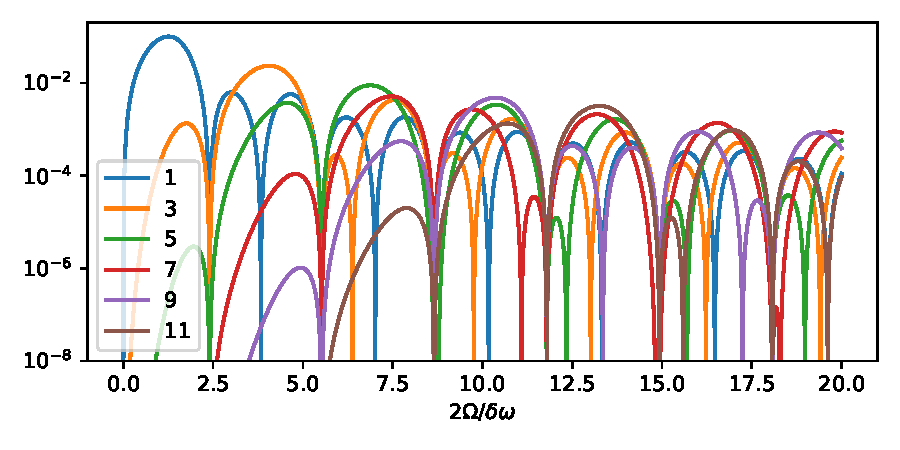
\includegraphics[width=0.95\textwidth]{zeros}
	\caption[Зависимость компонент эластичного рассеяния $I^{2l+1}(2\Omega/\delta\omega)$ для бихроматической накачки.]{Зависимость интенсивности компоненты эластичного рассеяния $I^{2l+1}(2\Omega/\delta\omega)$ для случая бихроматической накачки.}
	\label{fig: zeros}
\end{figure}
Подобную картину можно получить и при помощи рассмотрения одетого атома, однако в вышеупомянутых работах не приводится конкретных результатов для эластичного спектра, полученных на основе этого подхода. 

Мы рассмотрели известные теоретические и экспериментальные результаты для рассеяния бихроматического света на двухуровневой системе. По результатам рассмотрения можно отметить, что в данной работе впервые осуществляется систематическое экспериментальное исследование эластичного рассеяния: ранее в рамках традиционной оптики данный аспект изучался только теоретически, а известные экспериментальные работы \cite{Chakmakjian:88,Zhu_experiment} имеют дело только с неэластично рассеяным излучением. При этом, с точки зрения теории отдельно не рассматривался режим, в котором отстройка компонент драйва от резонанса кубита пренебрежимо мала по сравнению с излучательной шириной кубита.  Рассмотрев известные результаты, мы переходим к выполнявшимся в рамках работы экспериментам по рассеянию бихроматического света на одиночном сверхпроводящем кубите.
\section{Спектр эластичного рассеяния в случае $\delta \ll \Gamma_1$}
Исследование нелинейного рассеяния на одиночном кубите резонно начать с приложения к кубиту двух непрерывных волн. В рамках микроволновой техники наиболее просто использовать в качестве драйва выходные сигналы фазостабильных СВЧ-генераторов. В лаборатории искусственных квантовых систем для этого используются модели Keysight MXG N8257B и EXG N5283. Эти модели обеспечивают перестройку частоты в пределах до 20 ГГц, относительную аппаратную ширину линии порядка $10^{-11}$ и могут быть частотно синхронизированы друг с другом с такой же точностью. Кроме того, в качестве источника может использоваться и выход ВАЦ Keysight PNA-L, обладающий схожими характеристиками, но имеющий в качестве недостатка слабое подавление гармоник исходного синусоидального сигнала --- впрочем, этот эффект не является критическим для использования в обсуждаемом эксперименте. Для того, чтобы завести два непрерывных сигнала с различных источников в единый волновод, достаточно использовать СВЧ-делитель (splitter или power combiner) перед входом сигнала в криостат, объединенный выход которого направляется на вход криостата. Включение одного из источников позволяет произвести стандартные измерения однотоновой спектроскопии, зависимости линии кубита от мощности и резонансной флуоресценции, результаты которых рассматривались в разделах \ref{sec: spectr}-\ref{sec: Triplet_meas}. Нас же интересует спектр рассеянного на кубите сигнала, состоящего из двух компонент от разных источников.

Для решения поставленной задачи по измерению спектра эластичного рассеяния выход волновода с кубитом подключается к спектральному анализатору.  Зная естественную ширину его линии $\Gamma_1$, мы выбираем центральную частоту драйва $\omega_d$ близкую к частоте $\omega_q$ и устанавливаем на СВЧ-генераторах частоты $\omega_\pm = \omega_d \pm \delta\omega$, где величина отстройки $\delta\omega$ много меньше $\Gamma_1$, поскольку мы хотим остаться в резонансном приближении. Установив частоты, мы выравниваем мощности сигналов и начинаем синхронно увеличивать Раби амплитуды драйвов $\Omega_+ = \Omega_- = \Omega$, снимая получающийся спектр. При этом полоса входного фильтра спектрального анализатора может быть выбрана на уровне нескольких Гц, поскольку мы хотим максимально убрать шум и увидеть только эластичную часть сигнала, спектральная ширина которой очень мала.
\begin{figure}[thb]
	\centering
	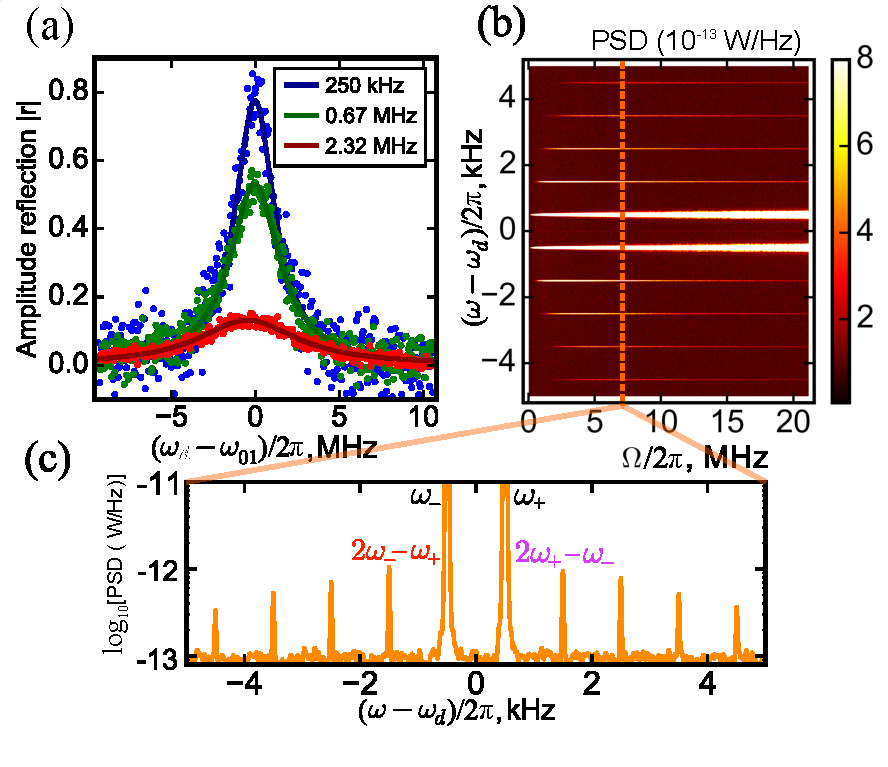
\includegraphics[width=0.85\textwidth]{Fig_2_fixed_PRA_forThesis.pdf}
	\caption[Волновое смешение: появление дополнительных компонент эластично рассеянного сигнала]{(a) Коэффициент прохождения $S_{21}$ одиночной резонансной волны на кубите в зависимости от отстройки $\Delta\omega = \omega_d-\omega_q$, при различных значениях частоты Раби. Параметры кубита $\Gamma_1/2\pi = 2.2$~МГц, $\Gamma_2 = \Gamma_1/2$. (b) Цветовой график спектров рассения двух волн на частотах $\omega_{\pm}$ в зависимости от частоты Раби для $\delta\omega = 1$ kHz. (c) Пример спектра при $\Omega/2\pi=7$~МГц. }
	\label{fig: CWM}
\end{figure}
Результаты измерений приведены на Рис.~\ref{fig: CWM}. Качественное поведение спектра по мере увеличения $\Omega$ хорошо проиллюстрировано на Рис.~\ref{fig: CWM}b). При увеличении Раби-частоты от нуля до нескольких единиц $\Gamma_1$ появляется большое количество эластичных пиков, частоты которых равны $\omega_{\pm(2p+1)} = (p+1)\omega_\pm-p\omega_\mp$ и интенсивности которых достигают своего максимума при определенных значениях $\Omega$, а в дальнейшем плавно спадают. Таким образом, экспериментально показан эффект волнового смешения непрерывных волн на одиночной нелинейности в волноводе. В данном измерении на пути сигнала не имеется никаких нелинейных элементов, которые мы могли бы вызвать подобное рассеяние. В качестве подтверждения, аналогичные измерения были проведены при большой отстройке кубита $\Delta\Omega = \omega_q - \omega_d \gg \Gamma_1 $, и в этом режиме не было обнаружено дополнительных спектральных компонент. Таким образом, можно считать доказанным факт наблюдения волнового смешения на одиночном сверхпроводящем атоме в волноводе.  

В режиме непрерывной бихроматической накачки интерес представляет снятие зависимость компонент напряжения, отвечающих дополнительным спектральным линиям, от частоты Раби $\Omega$, и сопоставить полученный результат с аналитическим расчетом. 



\section{Приближение малой отстройки}
прелюдия к расчету: пики от прецессии аналитического решения
\section{Аналитическое выражение для амплитуд боковых гармоник}
расчет и сопоставление
\section{Численное решение уравнений Максвелла-Блоха}
красивая большая картинка например про режим $\Omega \approx \delta \omega$
\section{Случай несбалансированных амплитуд}
 ну случай и случай